
\documentclass[12pt]{article}
\usepackage[latin9]{inputenc}
\setlength{\parskip}{\medskipamount}
\usepackage{textcomp}
\usepackage{amsmath}
\usepackage{graphicx}
\usepackage{epsfig}
\usepackage{vmargin}
\usepackage{setspace}
\usepackage[all]{xy}
\usepackage{multirow}
\usepackage{lscape}
\usepackage{hanging}
\usepackage{rotating}
\usepackage{array}
\usepackage{float}
\usepackage{rotfloat}
\usepackage[margin= 10pt, font=small, labelsep=period, skip= 0.5cm]{caption}
\usepackage{pdfpages}
\usepackage{abstract}
\usepackage{tablefootnote}
\renewcommand{\abstractnamefont}{\normalfont\Large\bfseries}
\newcolumntype{x}[1]{>{\raggedright \arraybackslash\hspace{0pt}}p{#1}}
\newcolumntype{y}[1]{>{\raggedright \arraybackslash\hspace{0pt}}m{#1}}
\newcolumntype{z}[1]{>{\centering \arraybackslash\hspace{0pt}}m{#1}}
\newcommand\Tstrut{\rule{0pt}{3.6ex}}       % "top" strut
\newcommand\Bstrut{\rule[-2.2ex]{0pt}{0pt}} % "bottom" strut
\newcommand{\TBstrut}{\Tstrut\Bstrut} % top&bottom struts
\renewcommand{\thetable}{\Roman{table}}
\providecommand{\tabularnewline}{\\}

% begin document-wide declarations

\setpapersize{USletter}
\setmargrb{1in}{1in}{1in}{1in}
\setlength\parindent{0.25in}
\pagestyle{plain}

% end document-wide declarations


\begin{document}


\title{Measuring the landscape of civil war:\\ \Large Evaluating geographic coding
decisions with historic data from the Mau Mau rebellion}

\author{\normalsize Dr. Rex W. Douglass\\
\normalsize Department of Political Science\\
\normalsize University of California, San Diego\\
 \\
 \normalsize Dr. Kristen A. Harkness\\
\normalsize  School of International Relations\\
 \normalsize University of St. Andrews\\
 \normalsize kh81@st-andrews.ac.uk} 
 
 \maketitle
\thispagestyle{empty}

\noindent \textbf{Abstract:} Subnational conflict research increasingly utilizes georeferenced event datasets to understand contentious politics and violence. Yet, how exactly locations are mapped to particular geographies, especially from unstructured text sources such as newspaper reports and archival records, remains opaque and few best practices exist for guiding researchers through the subtle but consequential decisions made during geolocation. We begin to address this gap by developing a systematic approach to georeferencing that articulates the strategies available, empirically diagnoses problems of bias created by both the data-generating process and researcher-controlled tasks, and provides new generalizable tools for simultaneously optimizing both the recovery and accuracy of coordinates. We then empirically evaluate our process and tools against new microlevel data on the Mau Mau Rebellion (Colonial Kenya 1952-1960), drawn from 20,000 pages of recently declassified British military intelligence reports. By leveraging a subset of this data that includes map codes alongside natural language location descriptions, we demonstrate how inappropriately georeferencing data can have important downstream consequences in terms of systematically biasing coefficients or altering statistical significance and how our tools can help alleviate these problems.\\ 

\noindent \textbf{Keywords:} georeferencing, archival data, civil war, Mau Mau, Kenya\\

\noindent \textbf{Acknowledgments}: We owe a debt of gratitude to Ali Puente-Douglass, Katherine Rember, and David Schaefer for research assistance at the British National Archives, Tom Scherer for coding assistance, as well as David Meyer and Erik Gartzke for feedback and institutional support. Earlier versions of this article were presented during a workshop at the 2016 annual conference of the Peace Science Society, at the Text Across Domains Symposium at U.C. Berkeley and at both the Machine Learning for Social Science Lab and the Center for Peace and Security Studies at U.C. San Diego. We thank the participants of these workshops as well as Laia Balcells, Christopher Sullivan, and three anonymous reviewers for their insightful comments and feedback.\newline

\noindent \textbf{Replication Data}: The data, codebook, and code for the empirical analysis in this article, along with the online appendix, can be found at https://github.com/rexdouglass/MeasuringLandscape. We provide R-Notebooks for each step of the analysis as well as a self-contained R package with all necessary code and data.\newline


\noindent \textbf{Biographical Statements:}\\

\noindent REX W. DOUGLASS, b. 1985, PhD in Politics (Princeton University, 2012); Assistant Project Scientist, University of California, San Diego (2016--- ); Director, Machine-learning for Social Science Lab, Center for Peace and Security Studies, University of California, San Diego (2016--- ); research interests: machine learning, natural language processing, and quantitative methods with applications to insurgency, civil war, and international security.\newline

\noindent KRISTEN A. HARKNESS, b. 1980, PhD in Politics (Princeton University, 2012); Lecturer, School of International Relations, University of St. Andrews (2013--- ); research interests: ethnicity and conflict in Africa with a particular focus on military institutions and democratization.\newline


\thispagestyle{empty}

\newpage{}\setcounter{page}{1}

\doublespace

\paragraph \indent How do we determine where historical acts of violence took place? At the heart of many questions in conflict studies is the where of violence: which areas were most violent? Where were civilians or communities targeted by conflict actors? Where did counterinsurgency tactics succeed or fail?  Underlying these analyses are decisions and assumptions about how to map events to the geography that they occupied.  Determining whether an event took place at a specific latitude and longitude, in a village or particular administrative unit, or somewhere else altogether is a matter of weighing evidence, comparing sources, and making judgment calls between different possible georeferencing strategies. Such important decisions, however, are usually made in an ad hoc manner, on the basis of opaque assumptions, and without the benefit of empirically tested guidance. 

We begin to address this gap by developing a systematic approach to georeferencing that articulates the strategies available, empirically diagnoses problems of bias created by both the data-generating process and researcher-controlled tasks, and provides new generalizable tools for simultaneously optimizing both the recovery and accuracy of coordinates.  We are able to do this by exploiting a new source of conflict data from the Mau Mau uprising in late colonial Kenya.  Drawn from over 20,000 pages of archival records, comprising raw intelligence reports written by British security personnel, our events contain either a natural language location description, a precise military map code, or both.  This allows us to explicitly test differences between georeferencing strategies and their relative performance by exploiting comparisons between imputed coordinates and the military coordinates.

The article proceeds as follows: the next two sections discuss existing debates over error and bias in spatial data and provide a brief survey of how georeferencing decisions are made across contemporary conflict research. We next introduce a new dataset of conflict events during the the Mau Mau rebellion, describing the archival records and how we sampled and coded them. We then discuss the tasks, decisions, and problems of georeferencing event data, including the trade-offs that various strategies entail for recovery versus accuracy. We also develop two new ensemble methods of georeferencing that leverage empirical diagnostic information to overcome these trade-offs, flexibly combining strategies and data sources to compensate for the weaknesses of any one. Finally, we empirically demonstrate how inappropriately georeferenced data can have important downstream consequences in terms of systematically biasing coefficients or altering statistical significance---and how our tools can help alleviate these problems.

\section*{Error and bias in spatial conflict event data}

\paragraph \indent Scholars have turned increasingly to analyzing subnational variation in protests, rebel violence, and repression. These works have transformed our understanding of contentious politics, allowing us to evaluate theories on the local dynamics of violence, the influence of terrain and infrastructure on war, and the myriad strategic interactions between states, their challengers, and civilians. This rigorous microlevel work depends on georeferenced conflict event datasets, which have proliferated in recent years. Regional or global event datasets include the Armed Conflict Location and Event Dataset (ACLED) (Raleigh et al., 2010), the UCDP Georeferenced Event Dataset (UCDP GED) (Sundberg \& Melander, 2013), and the Social Conflict in Africa Database (SCAD) (Salehyan et al., 2012), among others.\footnote{See also the University of Maryland's Study of Terrorism and Responses to Terrorism (START), the RAND Database of Worldwide Terrorism Incidents (RDWTI), the International Crisis Early Warning System (ICEWS), and the Global Data on Events Language and Tone (GDELT).} Intensive endeavors to compile georeferenced event data on particular conflicts have complemented such cross-national efforts (see Table I).


%Table 1: Single country georeferenced event datasets
\singlespace
\begin{table}
\centering \caption{Sample of single country georeferenced event datasets}
\begin{tabular}{x{2.65cm}x{5cm}x{7.5cm}}
\hline 
 \Tstrut Contemporary & Afghanistan 2004-11 & Berman et al. (2011); Lyall, Blair \& Imai (2013); O'Loughlin et al. (2010); Weidmann (2013)\\
   \Tstrut& Chechnya 2000-05 & Lyall (2009)\\
   \Tstrut& Columbia 1988-2000 &Albertus \& Kaplan (2012)\\
   \Tstrut& India 1984-96 &Hoelscher, Miklian \& Vadlamannati (2012)\\
   \Tstrut& Iraq 2004-10 &Berman et al. (2011); Berman, Shapiro \& Felter (2011); Condra \& Shapiro (2012); Shapiro \& Weidmann (2015)\\
   \Tstrut& Israel/Palestine 2000-05 &Benmelech, Berrebi \& Klor (2015)\\
   \Tstrut& North Caucasus 2000-08 &Toft \& Zhukov (2012); Zhukov (2012)\\
   \Tstrut& Northern Ireland 1968-1998 & Loyle, Sullivan \& Davenport (2014)\\
   \Tstrut& Pakistan 1988-2011 &Bueno de Mesquita et al. (2015)\\
   \Tstrut& Philippines 1997-2010 &Berman et al. (2011); Crost, Felter \& Johnston (2014, 2016)\\
   &&\\
  \Tstrut Historic & Greece 1943-44 & Kalyvas (2006); Kalyvas \& Kocher (2007)\tabularnewline
  \Tstrut& Guatemala 1975-1985 &Sullivan (2016)\tabularnewline
     \Tstrut& Spain 1936-39 &Balcells (2010)\\
        \Tstrut& Ukraine 1943-1955 &Zhukov (2015)\Bstrut\\
   \Tstrut& Vietnam 1965-75 &Douglass (2016); Kocher, Pepinsky \& Kalyvas (2011)\Bstrut\\ 
\end{tabular}
\end{table}
\doublespace

This increasing reliance on event data raises important questions over the data generating process and how systematic sources of bias could undermine valid causal inferences. Conflict event datasets never represent full `ground truth.' Rather, social actors with their own perspectives and agendas select events for observation, recording, and archiving (Woolley, 2000: 157). Journalistic sources, from which much event data has been coded, have come under heavy criticism for the small fraction of total events they capture, for coverage fatigue, and for bias towards large-scale, violent, and urban events (Baum \& Zhukov, 2015; Davenport, 2010: 7; Davenport \& Ball, 2002; Earl et al., 2004; Eck, 2012; O'Loughlin et al., 2010; Weidmann, 2016; Woolley, 2000). Archival records, on the other hand, are usually generated by government actors who have their own motives for collecting information during conflict. Indeed, they often selectively destroy or censor records and may systematically undercount civilian deaths resulting from their own operations (Balcells \& Sullivan, this issue).\footnote{For example, the British are thought to have destroyed countless records in their former colonies and hid hundreds of thousands more in a secret archive which was only recently discovered (Bennett, 2013: 3). In Pakistan, the U.S. government considers all military-age males killed in drone strikes as combatants unless their civilian status can be verified after the fact---an investigatory capability the U.S. clearly lacks (Byman, 2013: 36).}

Error and bias induced by the researcher controlled processes of data recovery, extraction, and coding have received far less attention.  Machine coding has been critiqued as a method of event compilation due to its apparently amplified urban bias and typical reliance on English language news sources (Hammond \& Weidmann, 2014; Wang et al., 2016). Scholars have also noted discrepancies in the spatial accuracy of datasets:  Eck (2012) finds UCDP-GED outperforms ACLED while Weidman (2015) demonstrates that both UCDP-GED and ACLED are highly inaccurate compared to U.S. military records from Afghanistan.  Branch (2016) also notes that georeferencing can introduce unrecognized problems with selection bias because it poorly captures non-spatial concepts that are then excluded or misrepresented in later analyses.

Although highlighting that georeferencing accuracy varies, existing work has not yet systematically analyzed how both the data generating process and researcher controlled decisions over measuring and modeling the landscape of civil conflict create their own biases and inefficiencies. Nor have we developed best practices in the field for how to rigorously georeference observations. This is the contribution we seek to make: how do we best extract locations from raw data and assign them coordinates? Georeferencing is a process of the researcher's own creation and under their control: while we cannot resolve all the myriad challenges arising from how records were generated, we can minimize our own contribution to bias and measurement error.
 

\singlespace
\section*{Contentious politics and existing approaches to geolocation}
\doublespace

\paragraph \indent Within the burgeoning microlevel literature on contentious politics, it has not yet become standard practice to describe georeferencing procedures such that they are fully transparent and replicable.  Even frequently used global event datasets such as the Global Terrorism Database (GTD) and the Global Database of Events, Language, and Tone (GDELT) fail to specify in their documentation exactly how coordinates were obtained from location names (toponyms).\footnote{See codebooks at https://www.start.umd.edu/gtd/downloads/Codebook.pdf and http://data.gdelt project.org/documentation/GDELT-Event\_Codebook-V2.0.pdf.} 

From those works that do describe their geolocation methods, three general practices can be discerned: reliance on GPS or satellite data, binning events into administrative units, or matching location names to coordinates through gazetteer databases. First, for some modern conflicts, GPS-enabled field equipment or satellite coverage provide highly accurate geographic information. The `Significant Activities' database was collected by U.S. soldiers in Afghanistan and Iraq with the technological capabilities to include GPS coordinates in their field reports (Berman et al., 2011; Berman, Shapiro \& Felter, 2011; Berman et al., 2013; Condra et al., 2010; Condra \& Shapiro, 2012; Gleditsch \& Weidmann, 2012; Shapiro \& Weidmann, 2015). Hassan \& O'Mealia (this issue) use satellite data to pinpoint arson events during the 2007-2008 Kenyan election violence. This type of geographical data is highly accurate and avoids the problems of later deriving coordinates from location descriptions. It is, however, also rare. Historic actors did not have such technological capabilities and even many contemporary governments (and other armed actors) do not have the resources, capacity, or will to collect GPS data in the field. There is also a very limited range to the types of data satellite imagery can capture.

More commonly, researchers forgo coordinates and bin events within existing administrative units. This is the case for much microlevel data collected on individual conflicts, including Chechnya (Lyall, 2009), Columbia (Albertus \& Kaplan, 2012), Pakistan (Bueno de Mesquita et al., 2015), Palestine (Benmelech, Berrebi \& Klor, 2015), the Philippines (Berman et al. 2011; Crost, Felter \& Johnston, 2014), Spain (Balcells, 2010), Ukraine (Zhukov, 2015), and Vietnam (Kocher, Pepinsky \& Kalyvas, 2011; Douglass, 2016). This approach avoids the problems of georeferencing while still reaching low levels of spatial aggregation, such as villages (although more commonly events are assigned to districts or municipalities). This practice, however, is non-ideal insofar as it compels the researcher to choose an administrative unit of analysis for practical reasons that may later conflict with theoretical needs or endogeneity concerns. Accurate and reliable conversion to coordinates would allow for greater flexibility over model specification, facilitate geographic matching and combination with other variables, and enable better use of data by future researchers driven by other questions.

Finally, a growing number of conflict event datasets match toponyms to coordinates through publicly available databases, such as the GeoNet Names Server or Google Earth, as well as historic gazetteers, field atlases, and other digitized maps.\footnote{ACLED, for example, uses a combination of the National Geospatial-Intelligence Agency's GeoNet Names Server (GeoNames), Google maps, Falling Grain, and other unspecified gazetteers (see codebook for Raleigh et al., 2010). UCDP-GED matches to GeoNames first then, failing that, consults Google Earth, followed by unspecified digitized maps and field atlases (Sundberg and Melander 2013, 526). SCAD works with a combination of Yahoo! Maps, Falling Grain, and www.itouchmap.com/latlong (see codebook for Salehyan et al., 2012).} Although the technical procedures remain opaque, it appears that most of these efforts begin with a primary database and then work sequentially through alternatives until a match is found between the location name and a set of coordinates. 

This haphazard approach poses a number of potential problems. First, it prioritizes recovery rates over accuracy by consulting sources of varying and often unknown quality until coordinates have been tracked down.  Second, it fails to systematically consider what the best match is out of a range of possibilities within and across databases. This creates unneccessary spatial error.  Third, manually consulting a broad range of databases and other sources of geographic information is highly labor intensive. Large amounts of data may then be left missing, especially for projects led by small teams of researchers.

Both missing coordinate data and spatial error are unlikely to be random. Georeferencing processes can thus carry over and create additional sources of bias that affect later analysis. This makes it vital to first render visible the important decisions made during georeferencing that affect the recovery rate, accuracy, and bias of coordinates. New tools are then necessary to assist the researcher in implementing the best georeferencing process for their event data, given its unique problems.


\singlespace
\section*{Best practices and new tools for building geographic conflict data}
\doublespace

\paragraph \indent The process of georeferencing, or matching textual descriptions of places to standardized identifiers (such as coordinates) through databases of geographic information (gazetteers), involves two fundamental concerns: precision (accuracy) and recall (recovery). Imprecision can seep into imputed coordinates through a wide variety of mechanisms: from errors in the data generating process that placed events far from their true locations, to mispellings or duplicated place names that lead to false matches, to errors in the underlying gazetteer data. The data generating process and georeferencing method can similarly affect recall rates. For example, records may give vague location information that is difficult to match to any gazetteer while some matching techniques, especially those requiring an exact match between location and gazetteer names, necessarily leave many observations missing.

If coordinates were truly missing at random, then low recall rates would simply reduce our sample size and downstream statistical leverage. Similarly, if inaccuracies were random, then low precision would merely introduce statistical noise and make relationships more difficult to discern, but would nonetheless return unbiased estimates. If the accuracy and/or missingness of coordinates are systematically distorted, however, then our later analyses would be subject to meaningful sources of potentially unacknowledged bias. 

It is therefore vitally important to understand how both the data generating process, in each unique context of data collection, and the georeferencing process create missing and/or inaccurate location information. Given this understanding, the researcher can tailor geolocation to minimize both its own problems and those that would otherwise carry over from the data generating process. Evaluating and implementing good strategies of georeferencing, in turn, rely on better tools that explicitly address the problems of precision and recovery and the potential trade-offs between them. 

The remainder of this section develops a systematic approach to georeferencing, including novel matching tools, with several benefits for the researcher. First, it eliminates the need to ex ante prioritize or exclude gazetteers, allowing the researcher to develop an individualized collection of sources that can be simultaneously consulted. Second, it systematically considers and derives best matches both within and across these sources, removing the labor intensive and somewhat haphazard task of trying to `hand match' locations to coordinates. Third, it provides flexible tools for maximizing recovery rates, minimizing inaccuracy, or balancing trade-offs between them. Fourth, it allows `self-referential' matching---or using coordinate locations included in the event observations themselves to provide matches for other observations missing this information.  Finally, it provides complete transparency in the subtle but meaningful choices that are usually opaquely left to the researcher (or research assistant) when trying to geolocate event data. 

A systematic approach to georeferencing involves four key choices, all of which potentially affect both recovery and precision (see Table II).  We discuss each of these choices in turn, giving recommendations for best practices or describing the trade-offs between options. We then present two new tools we developed to facilitate georeferencing according to these best practices.

%Table 2: Key Georeferencing Decisions
\singlespace
\begin{table}
\centering \caption{Key decision points in the georeferencing process}
\begin{tabular}{x{2cm}x{2.25cm}x{0.25cm}x{2.25cm}x{0.25cm}x{2.25cm}x{0.25cm}x{2.25cm}} 
\Tstrut Decision:&Which coordinate sources?&$\rightarrow$&Allow self-referential matching?\Bstrut&$\rightarrow$&Which geometry yype?&$\rightarrow$&Type of string matching?\\\cline{2-2}\cline{4-4}\cline{6-6}\cline{8-8}
\Tstrut Options:&single gazateer\Bstrut&&yes&&point&&exact\\
&sequentially consulted gazateers\Bstrut&&no&&polygon&&fuzzy\\
&combined gazateers\Bstrut&&&&multipolygon&&\\
&&&&&linestring&&\\
\end{tabular}
\end{table}
\doublespace

\emph{Which coordinate sources?}: First, the researcher must choose which gazetteers to use and how to potentially combine them. Not all gazetteers are created equal and, given the expanding number of available geographic information sources, the best are not readily apparent. For example, we found ten different coordinate sources for Kenya, ranging from historic gazetteers to government databases to commercial application programming interfaces (APIs) such as Google Earth and Bing Maps.\footnote{Kenya coordinate sources include: the 1964 Official Kenya Gazetteer; the U.S. Board of Geographic Names' database of foreign geographic feature names or NGA; the National Geospatial-Intelligence Agency's GeoNet Names Server or GeoNames; Google Maps' search API; Bing Maps' search API; OpenStreetMap; Global Administrative Areas database or GADM; Getty Thesaurus of Geographic Names; the International Livestock Research Institute; and Wikidata. Full source documentation is included in the online appendix.}  Instead of relying on general reputation (or even ease of access) to choose one data source, or to sequentially consult a small subset of sources, we recommend initially combining all data sources into a master gazetteer. This allows for diagnostics and comparisons of recovery rates and accuracy between gazetteers. It also enables the application of more sophisticated tools that can rank matches across gazetteers and suggest a best match for each individual observation. 

\emph{Allow self-referential matching?}: Datasets compiled from records that provide GPS or map coordinates, for at least some subset of observations, allow the researcher to engage in `self-referential matching.' By this we mean recovering coordinates for observations with only natural language location descriptions by matching them to other observations in the dataset rather than to external gazetteers. This practice can potentially greatly enhance recovery rates. Small rural locations, such as markets or farms, may not be included in global or even country-level gazetteers or may change names over time.  They may, however, be consistently referred to by conflict actors generating records in close temporal and spatial proximity. If, even once, such a location receives a coordinate in a document, then that geographic information can be recovered for all observations sharing the location name. The trade-off is that this practice will automatically spread any bias or error from these replicated coordinates throughout the dataset. One must thus carefully evaluate the underlying reliability of the actor-generated coordinates.

\emph{Which geometry type?}: Third, the researcher must choose the types of geometry to match on. The most common, point matching, treats locations as a single geographic point. Another possibility attributes polygons or multipolygons to locations and matches accordingly, which holds advantages for larger locations like towns and administrative units that we might feel uncomfortable reducing to a single point in space. Additionally, geographic features such as rivers can be treated as linestrings. Geometries can also theoretically be combined, assigning each location the point or shape with greatest verisimilitude. Different geometries may, however, involve trade-offs or sacrifices in recovery and accuracy and should be empirically judged within each context. 

\emph{Type of string matching?}: Finally, two general options exist to recover coordinates: exact matching and fuzzy matching. Exact matching requires an identical letter for letter match between toponyms in the event data and the gazetteer sources. The technique thus entails high precision (matches are likely true) but low recall. Indeed, many potential matches are missed due to minor deviations between sources, such as spelling errors, different prefixes and suffixes, and other modifiers (such as Aberdere National Forest versus Aberdere Forest). Intensive hand cleaning can partially overcome these disadvantages by fixing such discrepancies to the greatest degree possible; but recovery rates will nonetheless likely remain relatively low. Fuzzy matching, on the other hand, allows for toponyms to differ and still constitute a match, where the task is to carefully define the allowable degree of difference. Fuzzy matching thus has high recall, compared to exact matching, but may also generate many false matches, reducing precision.\footnote{Given the current lack of appropriate tools, we built a custom fuzzy toponym matching pipeline, treating it as a supervised learning problem. A full description of the pipeline and evaluation of its performance is provided in the online appendix. In brief, we created a training dataset of events with both text and military map codes paired against the ten closest gazetteer entries to the true location. We coded each event toponym-gazetteer dyad (n=20,243) as a match (3,192) or mismatch (17,051). A two stage classifier was then trained to predict the likelihood of a match between any two arbitrary toponym pairs. The first stage screened out pairs with little chance of being a match, using the Jaccard similarity between their 2-character ngram profiles, approximated with Locality Sensitive Hashing (LSH). A second stage then refined this smaller number of plausible matches using 28 different measures of similarity and estimated an exact probability with an XGBoost model.} The researcher must thus decide whether missing data or geospatial error is of greater risk to downstream analysis before choosing a string matching method. 

These choices often present trade-offs which are difficult to optimize across the entire georeferencing process. Ideally, we want to recover as many observations as possible, drawing across all available data sources and georeferencing methods, while still retaining precision.  To help achieve this, we developed two new tools that generate as many likely matches for as many observations as possible, while simultaneously sorting those suggestions by predicted accuracy. Below, we provide an intuitive insight into each tool with full technical details described in the online appendix.

\emph{Fixed hand rules ensemble}: This is an automated tool that requires the researcher to first evaluate which methods and gazetteers perform best, given their data, in terms of accuracy. Fixed rules are then programmed which tell the ensemble tool which matches to prioritize across observations. For example, we found that for our Kenya data exact matches were preferred to fuzzy matches, self-referential matches to gazetteer matches, and points to other geometric forms. We were also able to rank order our gazetteer sources by overall accuracy. Thus the tool was programmed to first generate possible matches across georeferencing strategies and then to select the one that best meets our customized preference ordering.

\emph{Semi-supervised ensemble}: While fixed rules are relatively easy to implement, they are inflexible and uniformly applied. This neglects additional information that could be used to pick the best possible match on a case by case basis, further minimizing imprecision and bias.  The semi-supervised ensemble treats georeferencing as a supervised learning problem, predicting how far away a potential match is from the true location.  This necessitates a moderately sized training dataset of ideal matches where observations have both a place name and known true location. This requirement may not be met by some datasets, especially those drawn exclusively from media sources. The model works by calculating the actual distance between known points and potential matches in the gazetteers, learning to predict this distance as a function of event and gazetteer properties such as reporting district, conflict year, data source, matching type, etc.

\footnote{We fit an XGBoost model, described later in the section `Choosing the right georeferencing approach for Kenya,' which predicts the log distance in kilometers between an event location and a gazetteer suggestion, minimizing mean squared error. Our unit of analysis is the event-gazetteer dyad (N=340,355) and the model includes the following independent variables: match properties such as the underlying gazateer source, spatial type, exact or fuzzy matching, and self-match; the predicted probability of a fuzzy match being true estimated with the second stage of the toponym matcher introduced above; place types from the gazetteers such as village, town, road, river, district, etc.; and document properties such as the reporting district and year.} The tool learns which potential match is likely to be the most accurate given all of this underlying information, flexibly applying its decision-making observation by observation.  This provides a more flexible approach than the fixed rules ensemble and is highly customizable given the unique needs and constraints of other geospatial data collection efforts. 


\singlespace
\section*{Application to the Mau Mau rebellion}
\doublespace

\paragraph \indent This sections employs our set of tools in the Kenyan context to, first, show how our data generating process created important biases that necessitated maximizing both recovered coordinates and their precision. Second, we give a proof of concept demonstrating how different georeferencing strategies create relative bias in how events are placed in relation to variables commonly thought to influence conflict dynamics---including population density and terrain ruggedness---and that those biases alter both coefficients and p-values when conducting simple hypothesis testing on the intensity of violence during the Mau Mau uprising. This particular dataset grants us vital leverage to evaluate and compare georeferencing strategies because it contains a subset of events with both natural language location descriptions and military generated map coordinates.

\singlespace
\subsection*{New data on the Mau Mau: The data generating process}
\doublespace

\paragraph \indent Best practices in constructing archival data, as recommended in the introductory article to this issue, require strong awareness of the data generating process and transparency in reporting it. How records were created, preserved, archived, and accessed creates potential sources of bias and determines the universe of events to which findings can legitimately speak. It is also recommended that researchers collect information using basic and unambiguous categories and highly disaggregated spatial and temporal units. This minimizes coder induced bias while preserving the fine-grained nature of the available records: categories and units can always be scaled up later in theoretically meaningful ways. Following these recommendations, we describe a new microlevel dataset on the Mau Mau uprising in late colonial Kenya (1952-1960). 

On 21 October 1952, in response to a string of murders and growing unrest, the colonial government of Kenya declared a State of Emergency.  Growing out of land grievances within the Kikuyu, Embu, and Meru (henceforth Kikuyu) tribal reserves, Mau Mau violence was targeted simultaneously at the colonial state, collaborating tribal chiefs and their locally recruited Home Guards, white settlers, and fellow Kikuyu who refused to participate in oathing ceremonies. These rituals were designed to silence the non-combatant population and bind their loyalty to the rebels.  While the armed forces battled guerrilla gangs in the forests, the native reserves turned into an intra-ethnic civil war, with much of the violence directed at Kikuyu non-combatants (Bennett, 2013: 12; Branch, 2009: 6; Furedi, 1973;  Kershaw, 1997: 212-247). Both sides were brutal: the government and its allies engaged in aerial bombardment, forced villagization, mass detentions, and extrajudicial torture and killings; and the insurgents routinely practiced targeted assassinations, massacres, arson campaigns, and the beating and murder of civilians (see Anderson, 2006; Bennett, 2013; Branch, 2009; Elkins, 2005).  The military phase of the Emergency ended in October 1956 when the last Mau Mau leader, Dedan Kimathi, was captured.  Emergency regulations and many tactics of pacification in the reserves were not lifted, however, until 12 January 1960.   According to official statistics, the conflict cost the lives of approximately 1,200 members of the Kenyan security forces (mostly Home Guard), 10,000-20,000 insurgents, and some 25,000 civilians (French, 2011: 151).\footnote{A sophisticated demographic study confirms that the total `excess deaths' amongst the Kikuyu was likely between 30,000-60,000 (Blacker, 2007: 225).} 

Conflict event data was recorded and compiled throughout the emergency by Special Branch, an intelligence unit within the police. Relying on the pre-conflict intelligence infrastructure of the colonial state, Special Branch officers assembled police and military intelligence from a wide range of sources into weekly, bimonthly, or monthly reports at the district and provincial levels. The purpose of these reports was to track conflict dynamics for local civilian and military administrators as well as for higher distribution to the wartime intelligence committees.   

Although the format varied across both time and space, each report contained some type of operational intelligence section with either a table of incidents or narratives of events. Because both police and military sources were consulted, a wide range of incidents were tracked, including both violent and non-violent events (oathings, theft, arson, abductions, assaults, killings, etc.). The incident lists also include government counterinsurgency activities, such as screening and sweep operations, patrols, and contacts between military units and rebels. Event descriptions include the date, location (often referenced with a military map code), a brief description of what occurred, and counts of arrested, wounded, and killed.

After the conflict, as decolonization approached, these files were removed from Kenya and buried from public view. It was only in 2011, following lawsuits filed against the United Kingdom's Foreign and Commonwealth Office\textemdash for torture committed during the Mau Mau uprising\textemdash that a hidden archive was discovered at Hanslope Park, Her Majesty's Government Communications Centre (Bennett, 2013: 3). Known as the `Migrated Archives' or the FCO 141- series, the records were deposited in tranches into the British National Archives at Kew between April 2012 and November 2013. They contain hundreds of thousands of pages of military and administrative documents detailing the violence that consumed late colonial Kenya.

Out of the massive volume of available documents, we sampled the Special Branch reports because of their comprehensive coverage.  Contained in 59 dossiers, the reports for the entire period of the Emergency have survived for most affected districts, with the exception of Fort Hall (missing after August 1954) and Machakos (missing after December 1955).\footnote{The intelligence files come from 16 districts as well as from Central Province, Rift Valley Province, and Nairobi City. The National Archives of the United Kingdom (TNA), Foreign and Commonwealth Office (FCO) 141/ 5721-22, 5726, 5730, 5733, 5736, 5746, 5751, 5754-62, 5766-82, 5784, 5786-88. 5791, 5793-94, 5827-33, 5839, 5841-43, 5846 \& 5850-52; also TNA War Office (WO) 276/378, 386 \&388.} Moreover, these reports and the intelligence infrastructure that compiled them both pre- and post-dated the uprising as well as existed in non-affected districts. We could thus rely on the content of the documents to tell us the geographic and temporal range of conflict events, instead of being subject to the government's judgment.\footnote{Despite the comprehensive coverage of the documents, some notable sources of potential bias remain. First, the intelligence records may not systematically capture major government operations in the heart of the forest zones, where the Mau Mau were encamped and civilians prohibited (these were outside district reporting boundaries). Second, because these records relied on military and police sources, they could undercount violent offenses by the government against civilians. Civilians would have been less likely to come forward with their experiences and security forces would have been less likely to document their own crimes. Finally, some Kenyan security forces were notorious for considering any man of military age caught outside his home area without proper papers, or in the act of running away, as a rebel. They also often deemed anyone they shot or injured as a rebel to protect themselves from investigation and possible prosecution for civilian abuses. We thus have low confidence that the data accurately distinguish between rebels and civilians.}

From the intelligence files, we coded 10,469 conflict events with nuanced information on the event and its location. We categorized each event by type and then coded both the instigator and target.  Data on casualties and captures was also extracted from the files, where available. Following best practices, we preserved as much disaggregation in the data as possible and used basic and unambiguous conceptual categories that can be aggregated into more theoretically driven concepts. For example, for the event type, coders were asked to extract brief original language descriptors from the event narratives summarizing the incident. We then pulled a list of all the unique descriptors from the compiled data and sorted them into basic categories before aggregating to larger concepts. The category `physical violence' thus includes the subcategories of `abduction' (`abduction' and `kidnapping'), `assault' (`assault' and `attack'), and `murder' (`murder' and `elimination'). The same process was followed for coding the instigator and target of the event.  This procedure allowed us to preserve a high degree of disaggregation and transparency, to avoid creating missing data by failing to appropriately specify categories ex-ante, and to minimize reliance on coder classificatory judgment.

\singlespace
\subsection*{Choosing the right georeferencing approach for Kenya}
\doublespace

\paragraph \indent Location information in our Mau Mau event data varies considerably. In the raw intelligence files, 51\% of observations are directly linked to precise military map codes under the East African Grid System.\footnote{We wrote code to convert these to modern coordinates in the WGS84 system, using instructions contained in United States Army Map Service 1944.} The precision of these coordinates is high, identifying events usually to within 1,000 meters of accuracy. 35\% of observations, however, only had natural language descriptions of the location and 14\% were missing location identifiers altogether, with only a reporting district noted (see Table 3).

%Table 3: Location information
\singlespace
\begin{table}[H]
\centering
\caption{Location information available from raw intelligence files}
\begin{tabular}{|l|cc|c|}
\hline 
&No Coordinates&Coordinates&Total\TBstrut\\
\hline
No Text Location&1,474 (14\%)&544 (5\%)&2,018 (19\%)\TBstrut\\
Text Location&3,663 (35\%)&4,788 (46\%)&8,451 (81\%)\TBstrut\\
\hline
Total&5127 (49\%)&5,332 (51\%)&10,469 (100\%)\TBstrut\\ 
\hline 
\end{tabular}
\end{table}
\doublespace

To understand whether underlying biases in the data generating process drove these differences, and how that should impact our georeferencing strategy, we modeled how both the properties of government data collection efforts (district, year, length of time window covered) and important attributes of the events themselves (initiator, target, and type of event) relate to location information. At several points, including here, we perform regression and classification tasks utilizing a non-parametric, machine-learning technique called Extreme Gradient Boosting (XGBoost) (Chen \& Guestrin, 2016) that works with both categorical and continuous independent variables. XGBoost is an ensemble method that iteratively fits individual models, with each new model designed to address the errors of proceeding models (called a greedy function approximator) (Friedman, 2001). The individual models comprise decision trees, which progressively split the data into smaller subsets similar in outcome as a function of the covariates. Each split represents a single cut on a single covariate. The trees are grown until reaching a stopping condition: a leaf node with only a single value on the outcome for classification and a leaf node with no less than three values for regression. For each observation, predictions from each tree are then weighted into a final prediction. To avoid over-fitting, each tree only has access to a random subset of observations and covariates. The majority of the technical discussion is relegated to the online appendix, including hyper-parameters, loss functions, training and test splits, cross validation, and class imbalance.

We find that events with military map codes are systematically different from those with only text descriptions. We fit a model that attempts to predict the likelihood of an event missing military map coordinates as a function of properties of that event. We find missingness to be nonrandom, with the model having high out of sample predictive accuracy (AUC 0.88).  Figure 1 shows how missingness varies with each covariate, measured as the predicted likelihood of missing map coordinates when setting a covariate to a specific value and holding all others at their observed value. The covariates are ordered top left to bottom right in terms of their measured importance to the overall model. Missing location information was most strongly related to the properties of the underlying intelligence document, suggesting that, when compiling any microlevel dataset, the unique data generating process of recording and preserving information is vital to understand. Certain kinds of reports, particularly those covering longer time periods and issued less regularly, were much less likely to contain exact coordinates compared to regularly issued weekly reports. Likewise, different years of the war were more likely to exclude spatial information than others. Reports from 1952, the first year of the Emergency, were about 40\% less likely to have coordinates than in 1955, probably reflecting disorganization as the state struggled to mobilize resources to counter the rebellion. The reporting district was also strongly predicted receiving a military map code. For example, events in the Fort Hall district files almost always contained specific coordinates while Nairobi city files nearly exclusively relied on textual descriptions. Provincial files and outlying districts from the conflict zone were also more likely to lack coordinates, with Machakos District around 75\% less likely to report map codes than Fort Hall. 

Lastly, we found variation in geographic reporting across action, target, and perpetrator of the event, with certain kinds of events in the war receiving systematically greater spatial coverage than others. Thefts and security operations were more likely to have coordinates than oathings or rebel captures. Events initiated by government actors, or against certain government actors (e.g. King's African Rifles and Police), were also more likely to have contain coordinates than others. Therefore, even though the government can give the appearance of capturing both sides of a conflict, the quality of that information may still vary systemically. How researchers choose to handle this missingness of spatial information will thus have important consequences for their analyses.

%Figure 1: Determinants of Missing Geographic Information
\singlespace
\begin{figure}
\centering
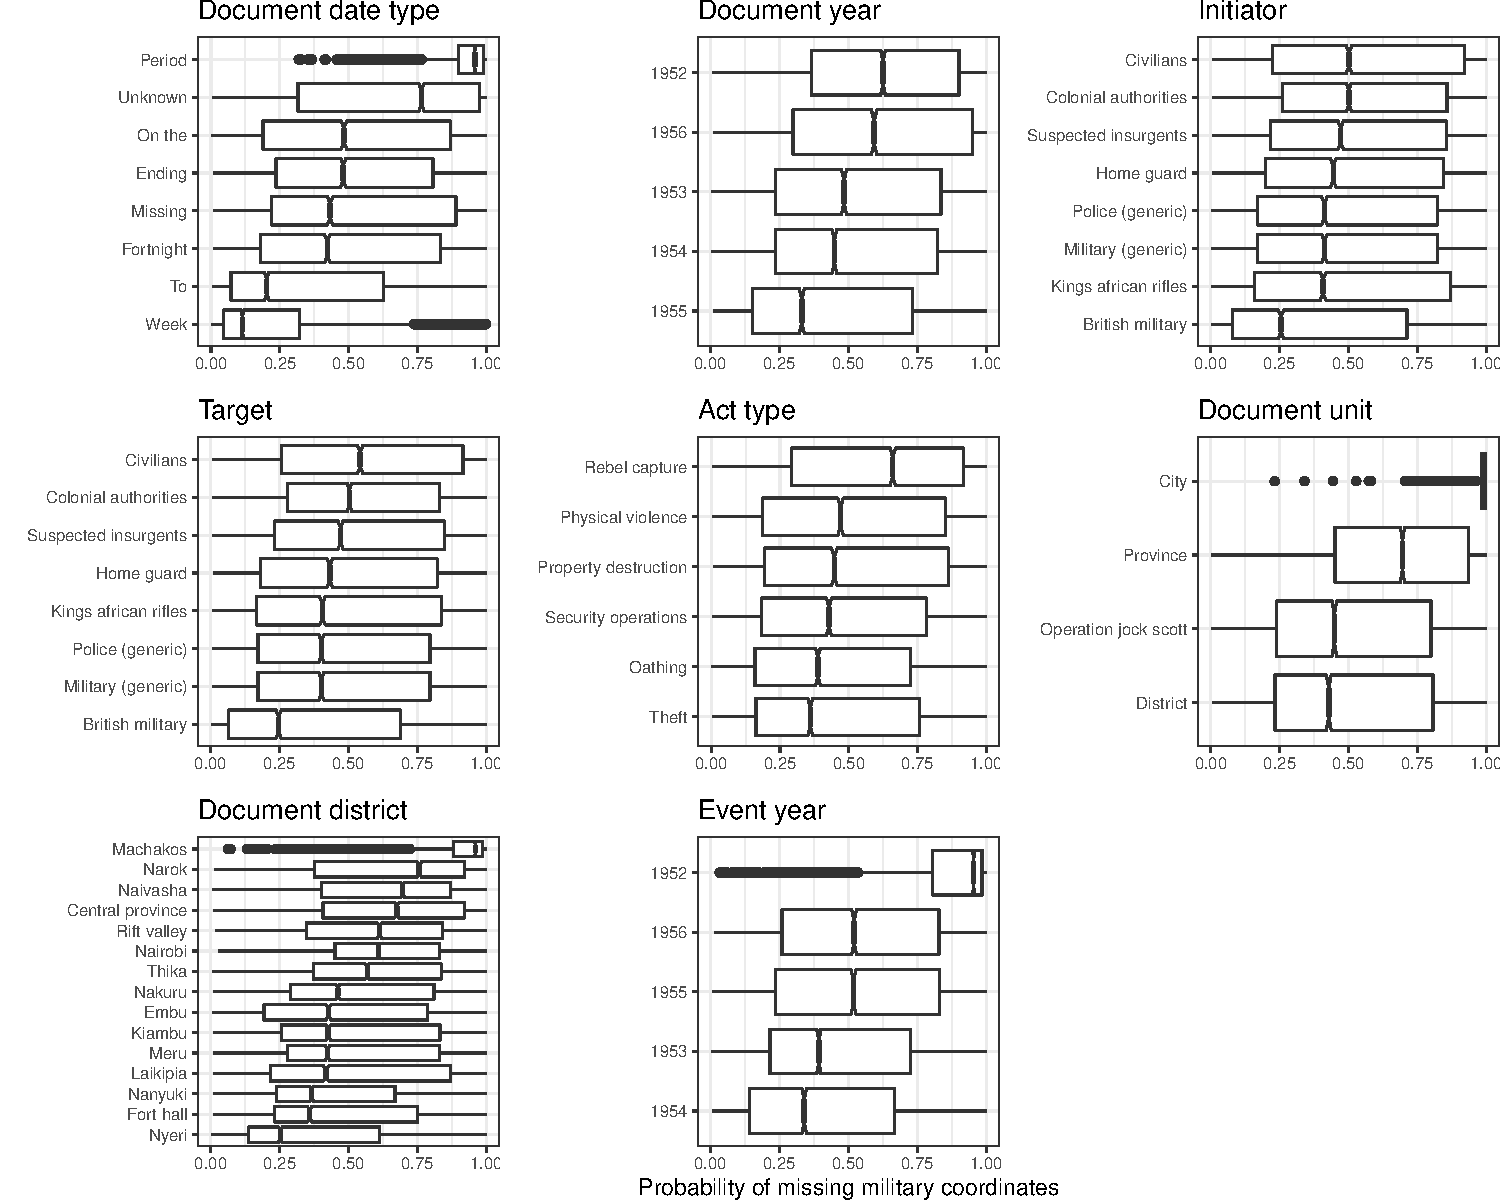
\includegraphics[width=6.5in]{rf_mapcoordinate_clean_missing.pdf}
\caption{Determinants of missing geographic information}
\caption*{Predicted probability of an event missing exact military coordinates as a function of the details of an event and the document properties (arranged by their relative predictive importance from top left to bottom right). The x-axis shows the probability of missing coordinates given a particular attribute of the event, holding all other properties to their observed values. Probabilities estimated with an XGBoost model. Missingness is non-random, with the model having high out of sample predictive accuracy (AUC of 0.88).}
\end{figure}
\doublespace


The data generating process in late colonial Kenya thus created serious sources of bias in the accuracy and missingness  of location information preserved by archival records. To drop observations without military map codes, or fail to recover a large percentage of them, would certainly bias later analysis. But so too would recovering a high volume of inaccurate coordinates, given the underlying processes that determined which events received map codes versus location names. To conduct downstream analysis, we were thus confronted with the pressing problem of simultaneously attempting to maximize recall and precision while geolocating events.

While this analysis is particular to the Mau Mau context, the same problems likely apply to many conflict settings. Simply omitting events with vague or missing location information would systematically undercount events from certain parts of the country and years of the conflict, which are often correlated with important patterns of spatial and temporal violence. It would also systematically undercount civilian and rebel initiated acts as well as certain categories of rebel behavior.

To maximize both accuracy and recovery of coordinates, we compared the performance of different georeferencing strategies and gazetteer sources, leveraging a subset of our observations that possessed both natural language location descriptions as well as reported military map codes. For each georeferencing technique and gazetteer, we graphed its recall rate against the mean squared error between the recovered coordinates and the military map codes. This evaluation required an untestable assumption: that the military map codes represent a close approximation to `ground truth' or the true location of events. Of course, soldiers in the field in the 1950s did not benefit from access to modern GPS equipment, which could introduce inaccuracies or biases into the military coordinates themselves. We think this is a minimal problem for two reasons: first, soldiers were working from high resolution local maps built from recently conducted aerial photography. They thus had reasonably good tools at their disposal to locate their own position, or incidents reported to them, using the natural features of the landscape, the road network, and nearby villages and farms. Second, the East Africa Grid System, in which they were working, used layered boxes to pin point positions which allowed soldiers to report map codes of varying levels of accuracy. If they were unsure of their precise location, they could use a slightly bigger box (and we do observe high volumes of both 7- and 9-digit map codes). Soldiers could also decline to use map codes altogether, as was often the case and likely to occur where grid coordinates would not improve upon simpler text descriptions. 

Figure 2 shows the relative performance of each individual gazetteer and georeferencing strategy along both dimensions of recall and precision. The upper left hand corner represents the choices that best meet our needs, maximizing recovery while minimizing  the distance to known military coordinates. The best performing gazetteers for our task are thus GeoNames, the NGA, and the historic 1964 Official Kenya Gazetteer. This was our most contemporary source of geographic information to the conflict itself, constructed from United Kingdom Survey of Kenya maps generated between 1953-1962. The Survey of Kenya maps were, in turn, based on aerial photography conducted in 1952 by the British Royal Air Force.\footnote{Kenya 1:50,000 series (Sheet 103/II), available through the British Library Maps at http://www.bl.uk/online gallery/onlineex/maps/africa/soomify136544.html.} Openstreetmap and Google, on the other hand, performed particularly poorly. With regard to georeferencing strategies, some choices were outright superior, while others involved important tradeoffs. Point matching, for example, outperformed all other types of geometry along both dimensions. On the other hand, exact matching maximized accuracy while fuzzy matching allowed for higher recovery rates. These results are unique to our data and would naturally vary in other contexts.

%Figure 2: Determinants of Missing Geographic Information (take off label on pdf; write caption; clarify key)
\singlespace
\begin{sidewaysfigure}
\centering
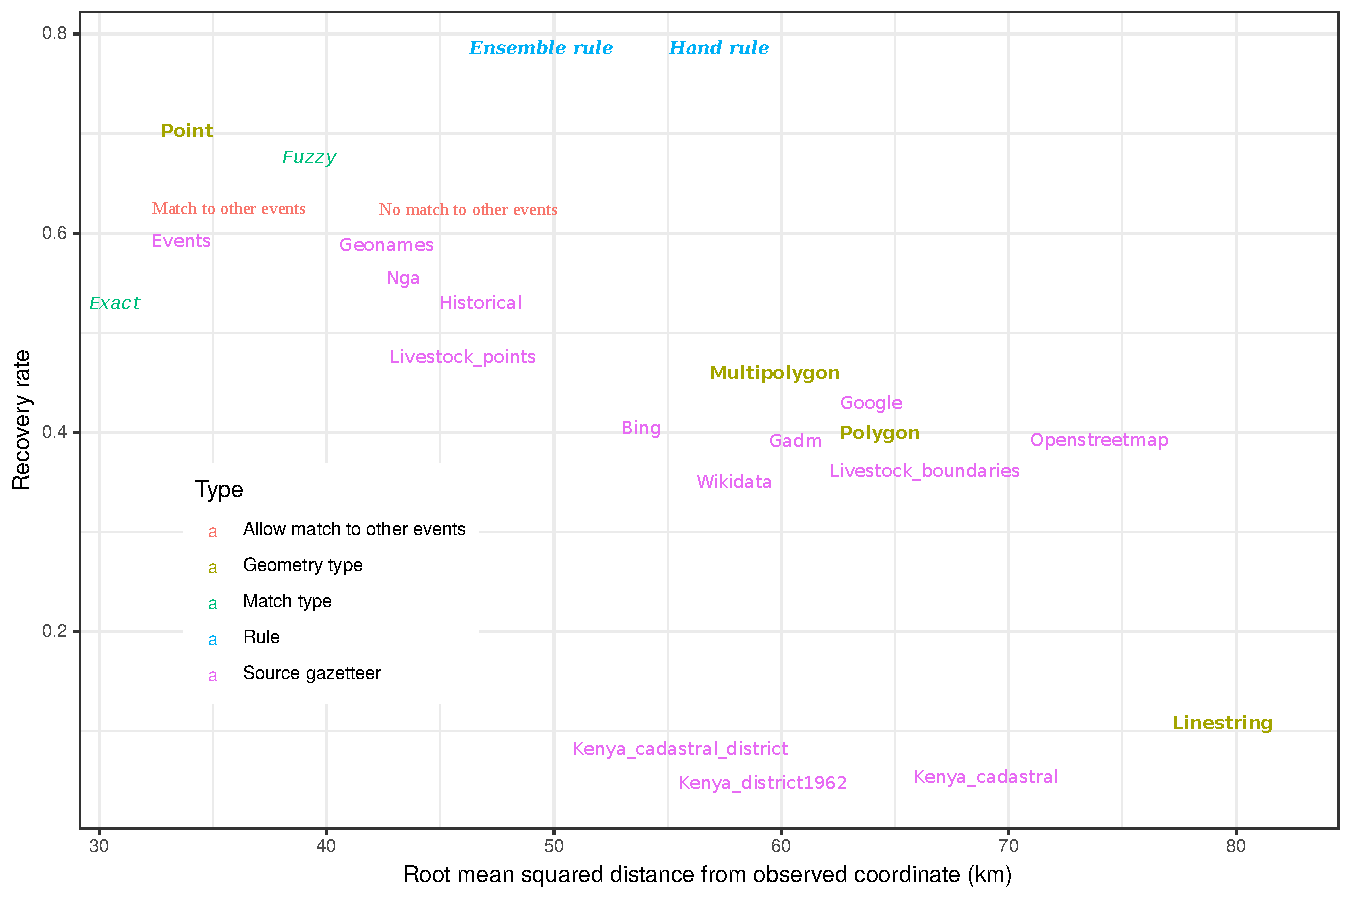
\includegraphics[width=8in]{RecallBias.pdf}
\caption{Comparison of recall and accuracy by georeferencing method}
\caption*{This figure shows how different georeferencing decisions vary in terms of recovery rate (y-axis) and accuracy (x-axis), measured by the root mean squared distance to the known military coordinates High recall and low spatial error (top left) is ideal, while low recall and large spatial error (bottom right) is to be avoided.}
\end{sidewaysfigure}
\doublespace


%Figure 3: Map of Georeferenced Kenya Event Data
\singlespace
\begin{figure} 
\centering
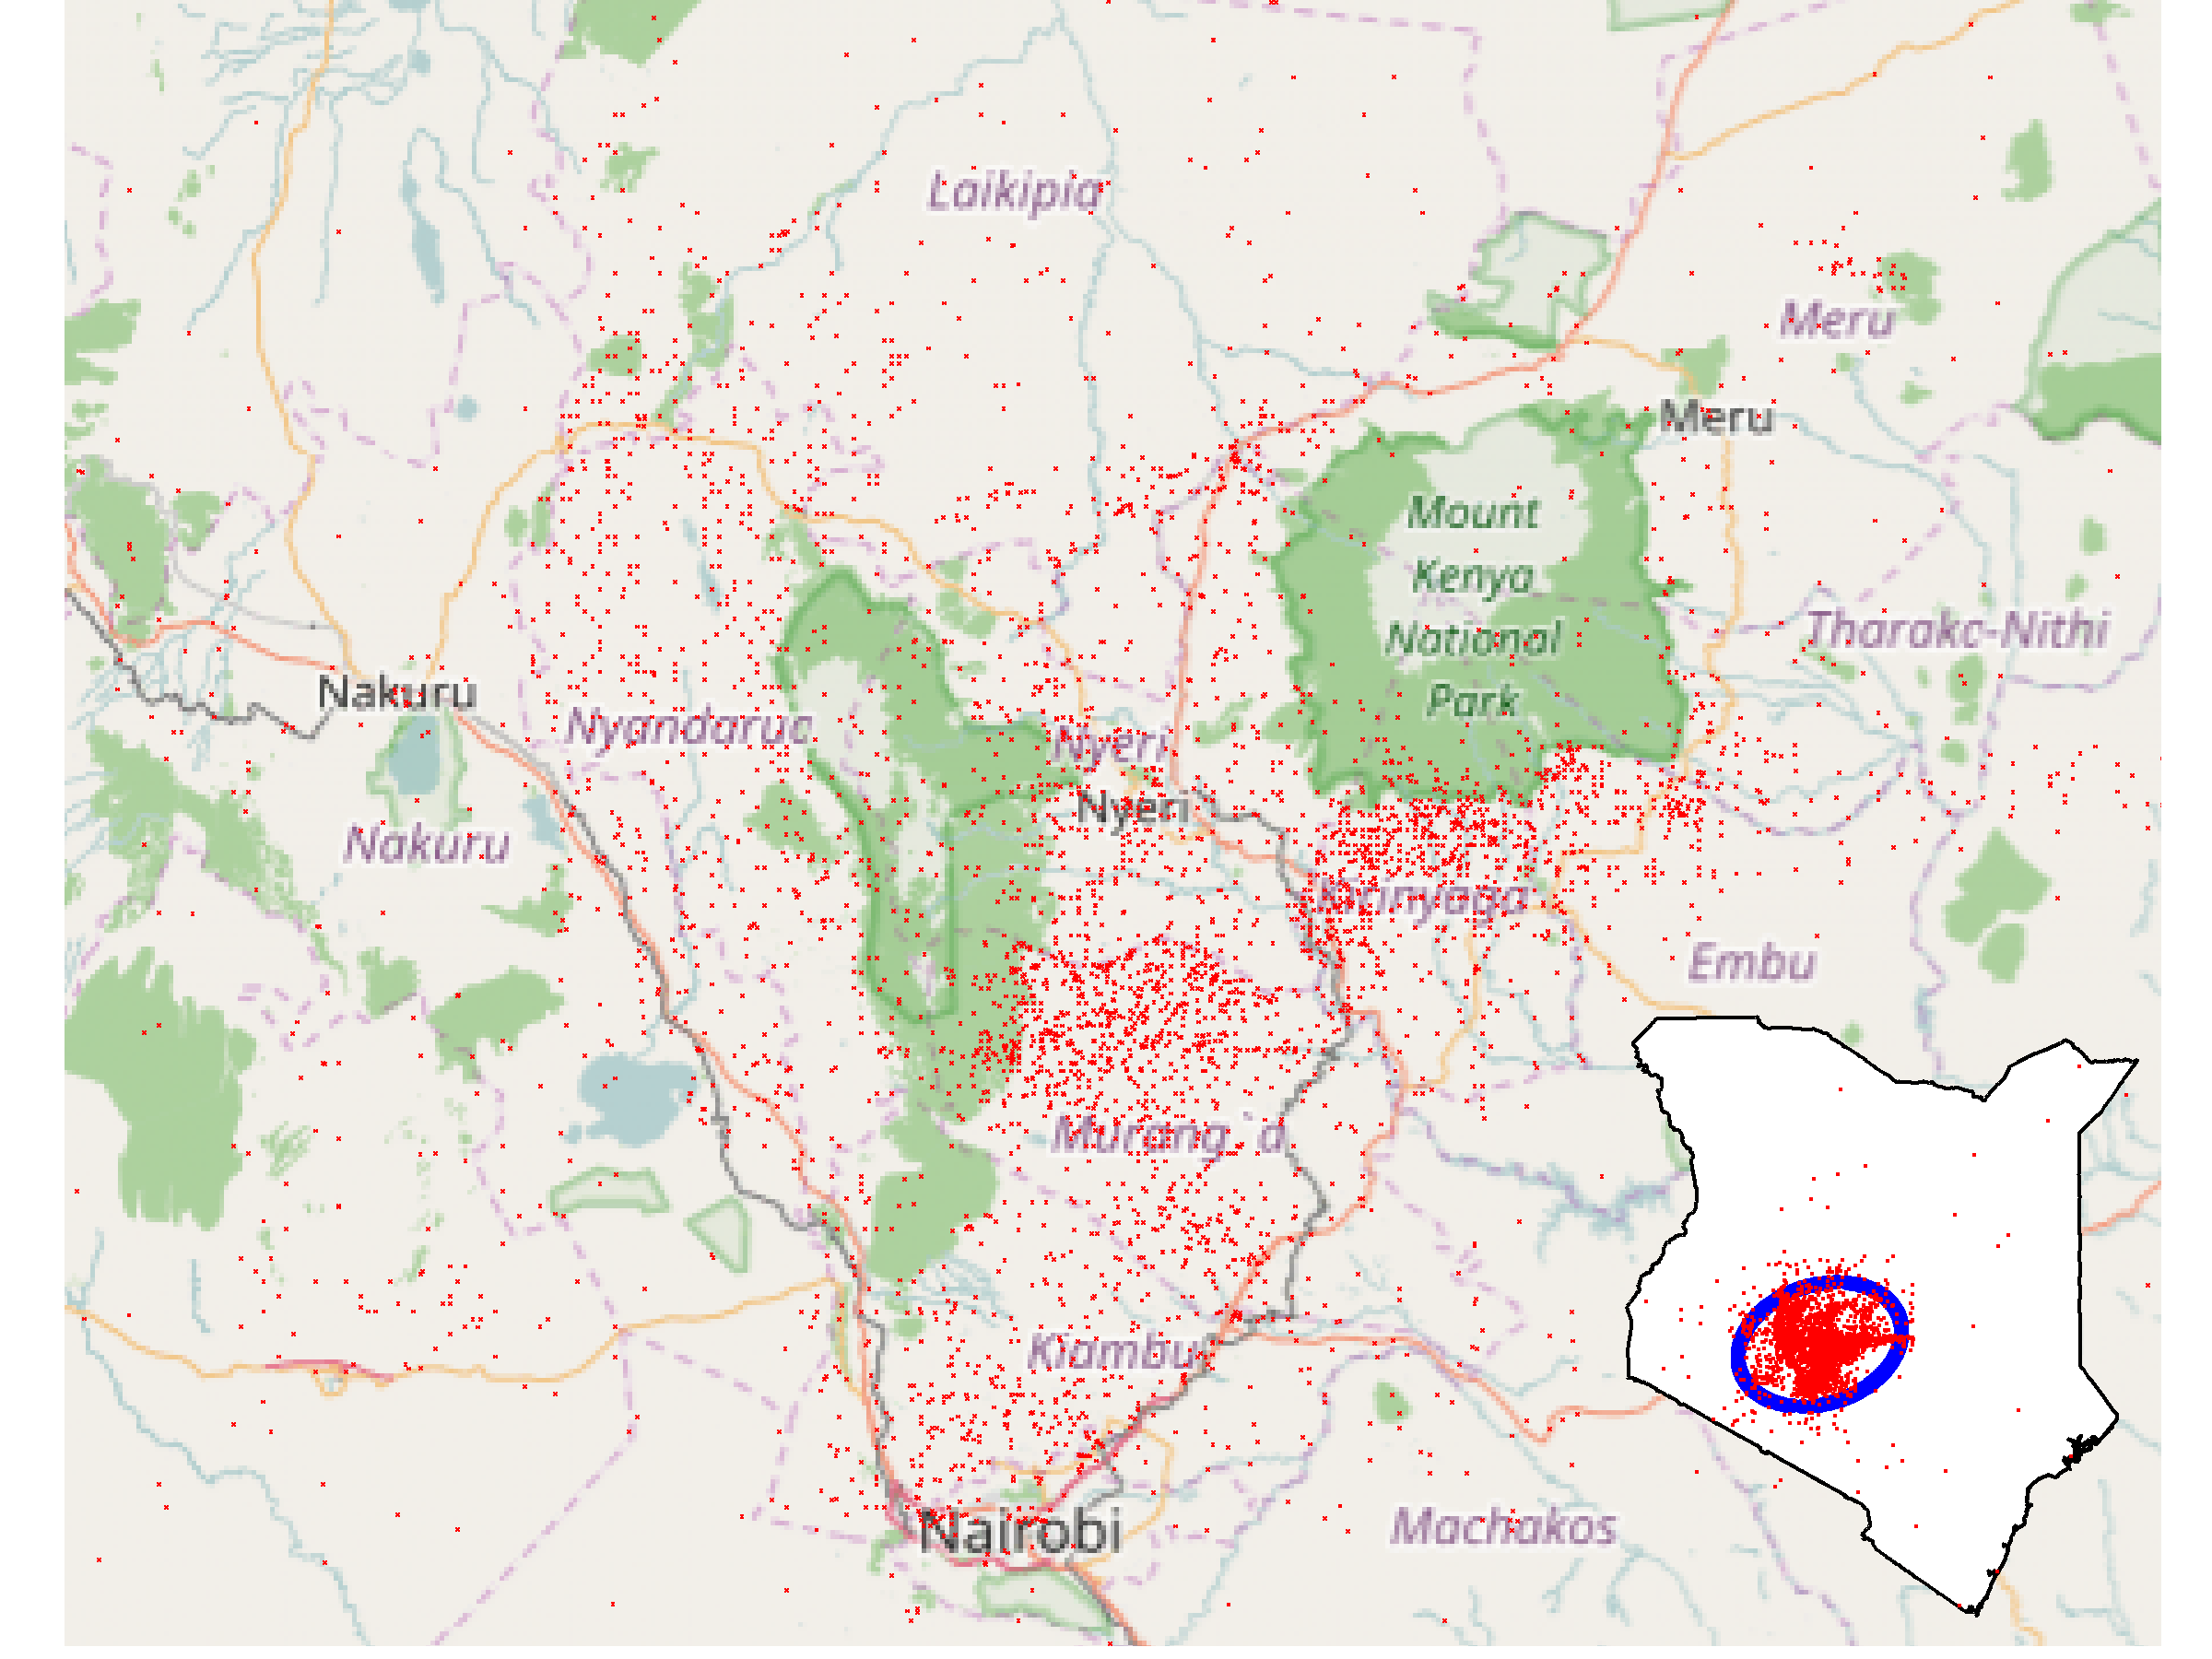
\includegraphics[width=6.5in]{p_openstreetmap_kenyamap.png}
\caption{Geographic distribution of Mau Mau conflict events}
\caption*{Region of interest with modern political features and place names. Individual conflict events represented by red dots. Inset shows modern international borders of Kenya with the region of interest contained within the blue ellipsis, estimated as a bivariate guassian containing 95\% of events.}
\end{figure}
\doublespace

Using these diagnostics, we then created preference orderings for the fixed rules ensemble. The semi-supervised ensemble also incorporated this information, as well as other observational attributes such as the reporting district, year, and report type as these were shown in the earlier analysis to structure missingness.  Figure 3 provides a map of our successfully georeferenced Mau Mau event data using the semi-supervised ensemble method, which could recover 71\% of observations. Both the hand based rules and the semi-supervised ensemble had comparable precision with root mean squared error of 31km and 30km respectively.

\singlespace
\section*{Proof of concept: Downstream consequences of geographic coding choices}
\doublespace

\paragraph \indent Paying close attention to the data-generating process, making informed choices over georeferencing methods, and following best practices should pay empirical dividends. Our data should be more reliable and less prone to bias than if we had made alternative choices. We test this in two ways. First, we analyze how different choices over gazetteers and georeferencing strategies generate relative bias in how close or far events are placed in relation to common variables of interest, including population density, distance from roads, and terrain ruggedness. Second, we examine how these same choices can bias coefficients or alter p-values in a simple hypothesis testing model with conflict intensity as the dependent variable. 

The first analysis once again rests on leveraging the subset of our observations that have both location descriptions and military map coordinates.  For each gazetteer, using the imputed coordinates, we calculate the average value of five commonly used independent variables and then compare them to the presumed `true values' generated by the military map codes. We chose distance to a road, density of forest cover, population density, volume of rainfall, and ruggedness of terrain as each of these variables is frequently employed in analyses of insurgency and contentious politics and claimed to impact patterns of violence (see Table 4 for variable descriptions and sources).  For example, security forces heavily utilize road networks, making them targets for IEDs and other attacks. Difficult terrain, such as dense forest cover and ruggedness, provide hiding places for insurgents, facilitating and prolonging conflict. Population centers provide large concentrations of targets as well as sources of supply and cover for insurgents blending into the civilian population.

We find that georeferenced locations are systematically different from coordinates provided by the military. Figure 4 shows the mean difference between imputed points and known military coordinates across each of the different gazetteer sources, organized by variable.  With rare exceptions, the various gazetteers placed events closer to roads (by about 25\%), in more populated areas (by about 30\%), and with less rainfall (by about 10\%). Perhaps more importantly, different gazetteers created distinct sources of bias both within and across variables. Ruggedness and forest cover, for example, varied significantly in the magnitude and direction of bias depending on the underlying source gazetteer. Users of event data, and consumers of the research based in it, have little ability to predict such biases and adjust inferences accordingly without conducting the diagnostics that we have. Additionally, to the degree that researchers wish to understand the role of these variables in producing or conditioning conflict events, careless or inappropriate georeferencing strategies could mechanically create relationships that will bias downstream analysis. 

%Table 4: Covariates
\singlespace
\begin{table}
\centering
\caption{Description of covariates}
\begin{tabular}{|y{3.5cm} z{3.5cm}|y{3.5cm} z{3.5cm}|}
\hline
\textbf{Variable}&\textbf{Spatial distribution}&\textbf{Variable}&\textbf{Spatial distribution}\\
\hline
\Tstrut \textbf{Population (log):} \small{persons living in a grid square (2km) in 1960, estimated based on national census data disaggregated by subnational political units (UNESCO, 1987).}\Bstrut&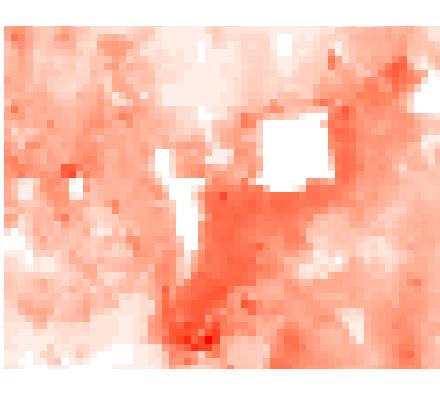
\includegraphics[width=1.25in,keepaspectratio]{p_pop.png} &\Tstrut \textbf{Distance to roads (log):} \small{road vectors digitized from contemporaneous road surveys (Colony and Protectorate of Kenya, 1951).}\Bstrut&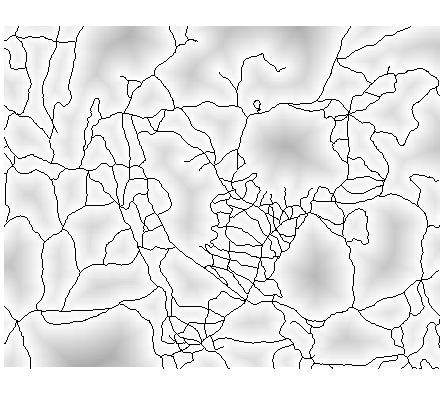
\includegraphics[width=1.25in,keepaspectratio]{p_roads.png}\\
\hline
\Tstrut \textbf{Ruggedness (log):} \small{measured as the square root of the squared absolute elevation between a 1 km cell and each of its contiguous neighbors (Shaver, Carter \& Shawa, 2016).}\Bstrut &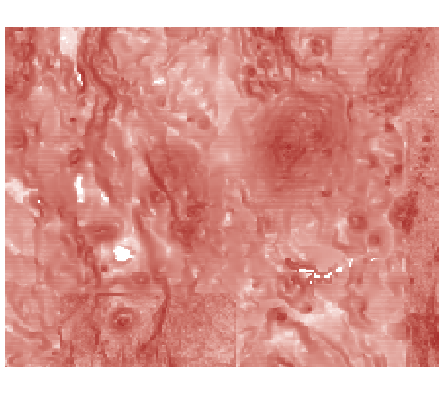
\includegraphics[width=1.25in,keepaspectratio]{p_rugged.png} &\Tstrut \textbf{Rainfall (log):} \small{average annual rainfall in mm (Hijmans et al., 2005).}\Bstrut&\includegraphics[width=1.25in,keepaspectratio]{p_rain.png} \\
\hline
\Tstrut \textbf{Forest cover:} \small{density of forest cover in 1km grid cells (Hansen et al, 2000).}\Bstrut&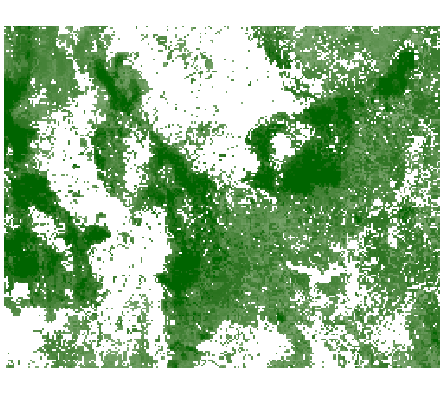
\includegraphics[width=1.25in,keepaspectratio]{p_forest.png}&&\\
\hline
\end{tabular}
\end{table}
\doublespace

%Figure 4: Bias in Georeferenced Data by Covariate 1
\singlespace
\begin{sidewaysfigure}
\centering
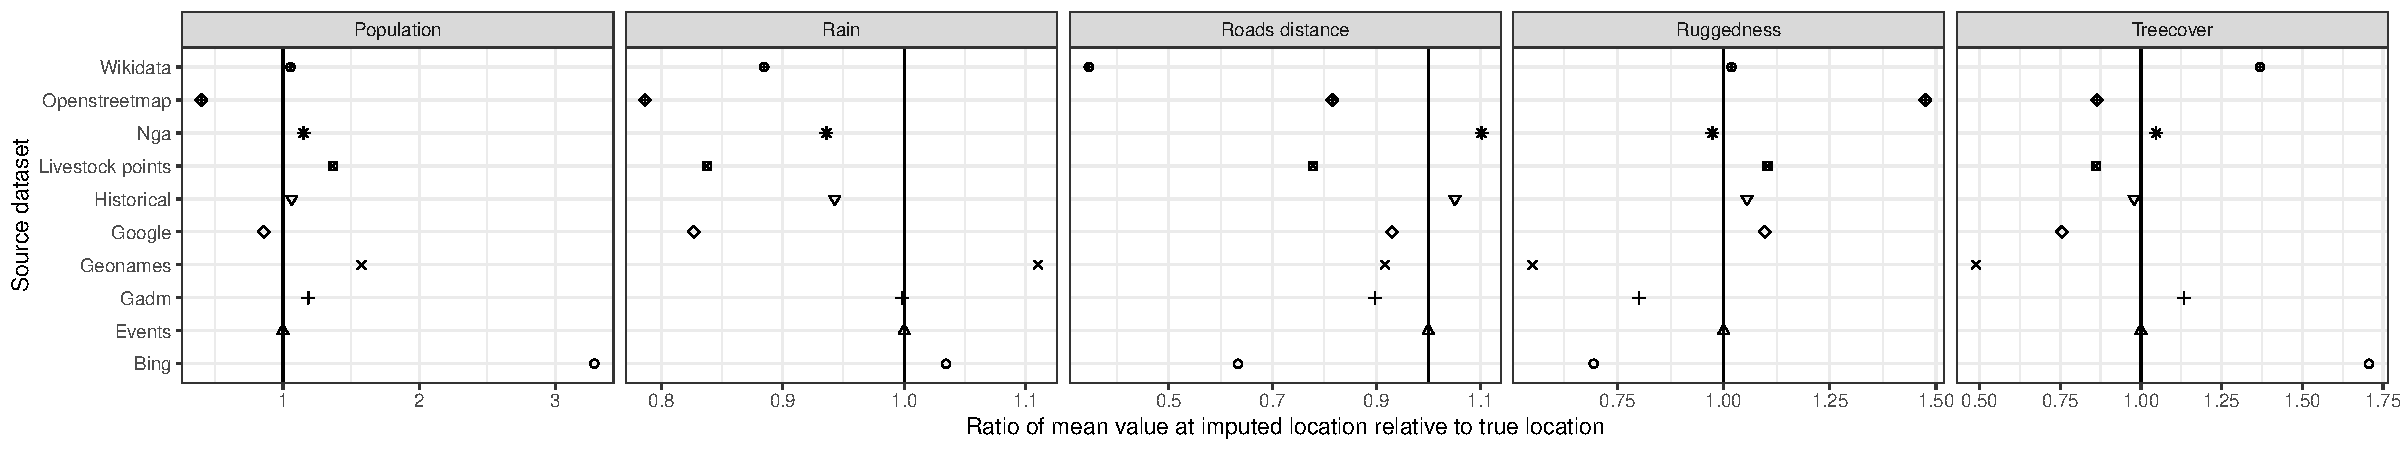
\includegraphics[width=8.5in]{p_bias_in_covariates_by_source.pdf}
\caption{Average absolute bias of georeferencing methods}
\caption*{Bias generated by different source gazetteers across five variables of interest to conflict studies. For each variable, the associated graph shows the mean absolute difference between imputed locations and the original military map coordinates, disaggregated by source gazetteer.}
\end{sidewaysfigure}
\doublespace


We now illustrate the impact of georeferencing decisions on a standard hypothesis testing model. We fit a negative binomial regression predicting the intensity of conflict in Kenya within a given geographic area (10km wide hexagons) as a function of our five independent variables (population, rainfall, distance from roads, ruggedness, and forest cover). Not only are these variables routinely included in conflict models, but they have particular relevance to the Kenyan context. The Mau Mau maintained their bases high up in the Aberderes and Mt. Kenya forests and were targeted there by government security forces, both by ground troops and aerial bombardment (Anderson, 2005: 230-288). Much of the conflict, however, likely occurred at the borders between the forests and the settled area as rebel bands ventured down, seeking supplies and support from the civilian population. It was here that they came into contact both with loyalists and with patrolling security forces (Bennett, 2013: 20-26). For similar reasons, population density also likely shaped the dynamics of violence as the heavily populated Kikuyu tribal reserves became a battleground between the Mau Mau and the local defense forces, with civilians and their loyalties caught in between (Branch, 2009: 55-93). The road network served as an artery of security force patrols, potentially enhancing population security closer to paved roads but also providing a target for rebel attacks. Finally, rainfall directly impacts agricultural quality and the productivity of land. Since Mau Mau arose over land disputes and the growing wealth disparities both within the Kikuyu community and compared to the white settle population, we might expect more conflict events around highly productive land (Kershaw, 1997: 212-241).%add citations   

We fit a multitude of models, varying only the gazetteers and georeferencing strategy.\footnote{Which does change the universe of observations and degree of spatial missingness depending on what each method recovers.} Results are shown in Figure 5, which plots the coefficients (exponentiated) on the X-axis and the p-value on the Y-axis for each variable. This allows one to visualize shifts in both statistical significance and substantive meaning across georeferencing decisions.

%Figure 5: Regression Results across Georeferencing Choices
\singlespace
\begin{sidewaysfigure}
\centering
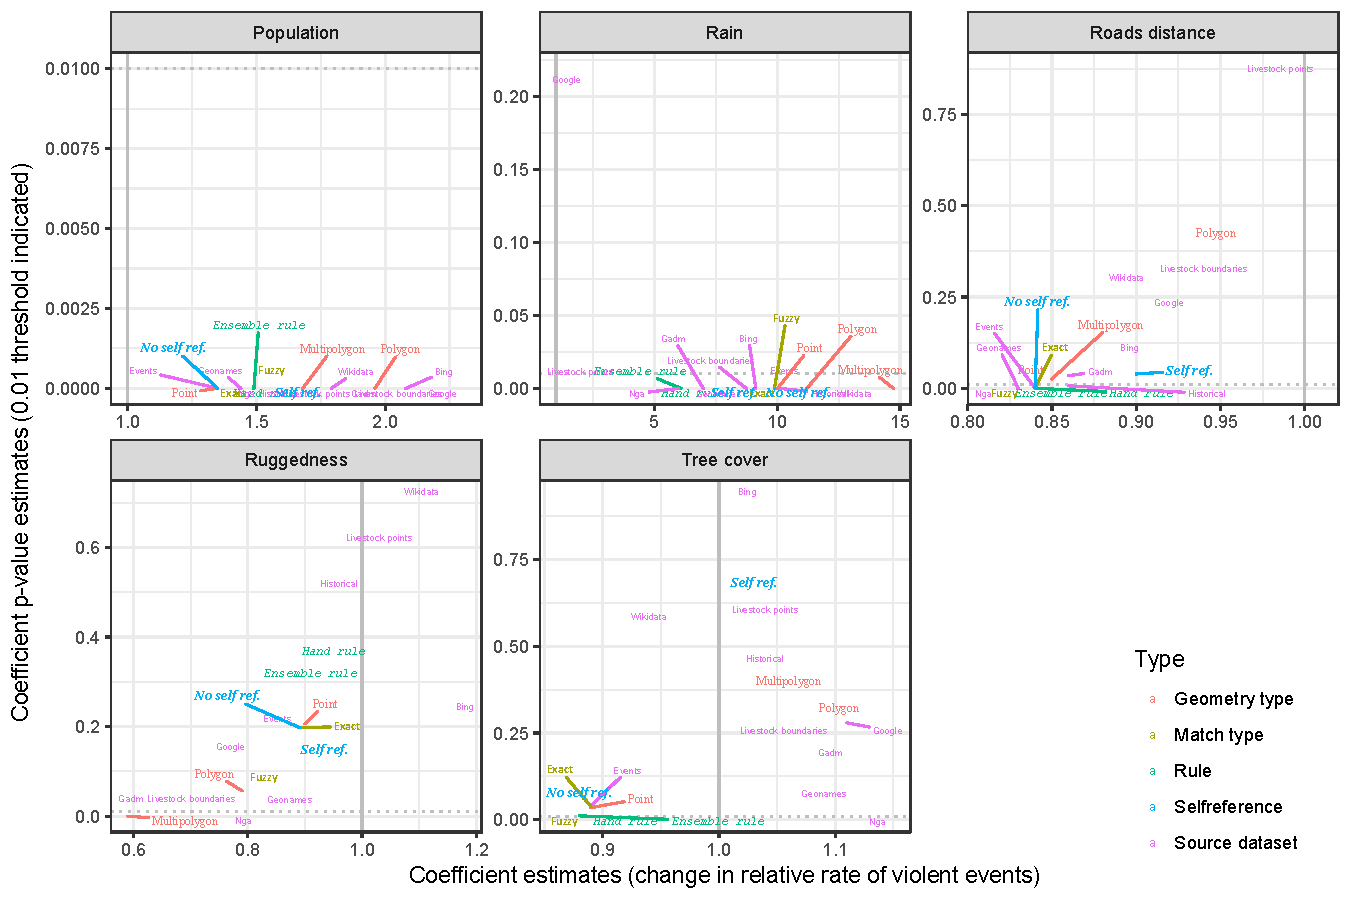
\includegraphics[width=8in]{p_lm.pdf}
\caption{Regression results across georeferencing choices}
\caption*{This figure shows coefficient estimates from a negative binomial regression model predicting the count of events occurring in 10km hexagon bins as a linear function of five covariates and an error term. Each box represents a single covariate and displays how the p-value (y-axis) and exponentiated coefficient (x-axis) shift as different georeferencing strategies and source gazetteers are used to construct the underlying data prior to spatial binning. Three outliers take extreme values, primarily because of low recovery rates, and are not shown. Statistical significance as well as the magnitude and direction of the coefficients all vary as a result of different georeferencing decisions.}
\end{sidewaysfigure}
\doublespace

Even in this simple model with few covariates, we find wide variation in substantive effect, significance, and sign across the georeferencing strategies. Population and rainfall demonstrate the least ambiguous effects, their coefficients uniformly positive (with one exception) and always statistically significant. The magnitude of their coefficients, however, ranges greatly: a one unit increase in log population creates anywhere from a 1.5 to 3 fold increase in conflict intensity while the same increase in log rainfall generates 8 to 30 times as many conflict events. All results thus support the understanding that more highly populated communities on good land were disproportionately impacted by the conflict; how disproportionately varies by the georeferencing method. Distance from roads also consistently decreases conflict intensity across models, although there is wide variation on whether the effect gains statistical significance. Depending on our georeferencing strategy, we might thus conclude that roads fail to matter or that police and military patrols facilitated by paved roads greatly improve security, at least in this context. Finally, the results for ruggedness vary drastically in terms of statistical significance and the sign of the coefficient even flips for several gazetteer sources. Tree cover is also severely impacted, with no consistency in the sign, magnitude, or statistical significance of the coefficient. Given the importance of forests and mountains to both rebel and government strategies in the Kenyan context, this is worrisome indeed. Getting the georeferencing wrong would prevent us from generating valid inferences on a central dynamic of this conflict.

\singlespace
\section*{Conclusion}
\doublespace

\paragraph \indent Microlevel conflict analyses involve a host of typically hidden decisions over how to handle the spatial components of event data, beginning with the georeferencing process itself. We demonstrate that these choices have clear consequences for downstream analysis, including the validity and interpretation of statistical results. Yet, no clear best practices currently exist in the field to guide the complex process of mapping events to their geographies.

This article attempts to fill this void, leveraging original data on the Mau Mau rebellion to flush out the decision making process of retrieving coordinates while developing new tools for maximizing recovery and minimizing error and bias. We demonstrate diagnostics that can be used to understand the data generating process and how the social actors who recorded and archived events introduced systematic bias into geographic missingness. We also provide simple, empirically informed guidelines on the decisions that must be made during georeferencing and the tradeoffs they entail. Finally, we introduce machine learning based methods to overcoming the weaknesses of any particular data source or georeferencing choice. Our ensemble tools allow for the sophisticated combination of gazetteers while discerning best probable matches given the underlying features and empirically discovered problems of the data.These tools can be adapted to any conflict where at least a portion of the location descriptions can be reasonably linked to known, accurate coordinates.

Of course, our tools do have limitations of which researchers should be aware. To conduct the diagnostics and generate appropriate hand rules as well as to properly train the semi-supervised ensemble, one needs a subset of the data with a reasonably accurate `ground truth.' For media-based events, this could be constructed by analyzing  potential overlaps with GPS-based military records (such as the Significant Activities data for Iraq and Afghanistan). For historic conflict data, one would likely be reliant on the archival records themselves to provide this sample (as many British records do). Machine learning techniques also require more technical expertise and computational costs than current approaches to georeferencing.

Our findings also suggest a number of important insights for both producers and consumers of conflict event data. At a minimum, there needs to be greater transparency and documentation of the steps taken during georeferencing. When multiple strategies are available, the chosen one should be theoretically and empirically justified. Ideally, alternative georeferencing decisions would be explored and included in the data release, enabling sophisticated robustness checks. Our analysis also indicates that all users of event data should be highly cognizant of the data generating process.  The historical record is a product of the decisions, incentives, and constraints of individuals and institutions, who are  themselves embedded in the social processes they have documented. At a minimum, we must try to understand the underlying biases in our data and not magnify their effects. With sophisticated tools, as we have tried to develop, we may even be able to mitigate such biases.

%Bibliography

\newpage
\noindent \textbf{\Large{References}}\\
\singlespace \begin{hangparas}{.25in}{1}

\par Albertus, Michael \& Oliver Kaplan (2012) Land reform as a counterinsurgency policy: Evidence from Columbia. \emph{Journal of Conflict Resolution} 57(2): 198-231.\newline

\par Anderson, David (2006) \emph{Histories of the Hanged: Britain's Dirty War in Kenya and the End of Empire}. New York: W.W. Norton \& Company, Inc.\newline

\par Balcells, Laia (2010) Rivalry and revenge: Violence against civilians in conventional civil wars. \emph{International Studies Quarterly} 54(2): 291-313.\newline

\par Baum, Matthew A \& Yuri M Zhukov (2015) Filtering revolution: Reporting bias in international newspaper coverage of the Libyan civil war. \emph{Journal of Peace Research} 52(3): 384-400.\newline

\par Benmelech, Efraim; Claude Berrebi \& Esteban Klor (2015) Counter-suicide-terrorism: Evidence from house demolitions. \emph{Journal of Politics} 77(1): 27-43.\newline

\par Bennett, Huw (2013) \emph{Fighting the Mau Mau: The British Army and Counter-Insurgency in the Kenya Emergency}. Cambridge: Cambridge University Press.\newline

\par Berman, Eli; Michael Callen, Joseph H Felter \& Jacob N Shapiro. (2011) Do working men rebel? Insurgency and unemployment in Afghanistan, Iraq, and the Philippines. \emph{Journal of Conflict Resolution} 55(4): 496-528.\newline

\par Berman, Eli; Jacob N Shapiro \& Joseph H Felter (2011) Can hearts and minds be bought? The economics of counterinsurgency in Iraq. \emph{Journal of Political Economy} 119(4): 766-819.\newline

\par Blacker, John (2007) The demography of Mau Mau: Fertility and mortality in Kenya in the 1950s: A demographer's viewpoint. \emph{African Affairs} 106(423): 205-227.\newline

\par Branch, Daniel (2009) \emph{Defeating Mau Mau, Creating Kenya: Counterinsurgency, Civil War, and Decolonization}. Cambridge: Cambridge University Press.\newline

\par Branch, Jordan (2016) Geographic information systems (GIS) in international relations. \emph{International Organization} 70(4): 845-869.\newline 

\par Bueno de Mesquita, Ethan; C Christine Fair, Jenna Jordan, Rasul Bakhsh Rais \& Jacob N Shapiro (2015) Measuring political violence in Pakistan: Insights from the BFRS dataset. \emph{Conflict Management and Peace Science} 32(5): 536-558.\newline

\par Byman, Daniel (2013) ``Why drones work: The case for Washington's weapon of choice. \emph{Foreign Affairs} 92(32): 32-43.\newline

\par Chen, Tianqi \& Carlos Guestrin (2016) Xgboost: A scalable tree boosting system. \emph{Proceedings of the 22nd ACM SIGKDD International Conference on knowledge, discovery, and data mining}: 785-794.\newline

\par Colony and Protectorate of Kenya (1951) Key plan of road maps of the colony prepared to scale 1:500,000. Nairobi: Road Engineers Office Public Works Department. Obtained from The National Archives (Kew) Colonial Office 1054/122.\newline

\par Condra, Luke N \& Jacob N Shapiro (2012) Who takes the blame? The strategic effects of collateral damage. \emph{American Journal of Political Science} 56(1): 167-187.\newline

\par Crost, Benjamin; Joseph Felter \& Patrick Johnston (2014) Aid under fire: Development projects and civil conflict. \emph{The American Economic Review} 104(6): 1833-1856.\newline

\par Crost, Benjamin; Joseph Felter \& Patrick Johnston (2016) Conditional cash transfers, civil conflict and insurgent influence: Experimental evidence from the Philippines. \emph{Journal of Development Economics} 118: 171-182.\newline

\par Davenport, Christian (2010) \emph{Media Bias, Perspective, and State Repression: The Black Panther Party}. Cambridge: Cambridge University Press.\newline 

\par Davenport, Christian \& Patrick Ball (2002) Views to a kill: Exploring the implications of source selection in the case of Guatemalan state terror, 1977-1995. \emph{Journal of Conflict Resolution} 46(3): 427-450.\newline

\par Douglass, Rex W (2016) Understanding civil war violence through military intelligence: Mining civilian targeting records from the Vietnam War. In C.A. Anderton \& J. Brauer (eds.) \emph{Economic Aspects of Genocides, Mass Atrocities, and Their Prevention}. New York: Oxford University Press.\newline

\par Earl, Jennifer; Andrew Martin, John D McCarthy \& Sarah Soule (2004) The use of newspaper data in the study of collective action. \emph{Annual Review of Sociology} 30: 65-80.\newline

\par Eck, Kristine (2012) In data we trust? A comparison of UCDP GED and ACLED conflict event datasets. \emph{Cooperation and Conflict} 47(1): 124-141.\newline

\par Elkins, Caroline (2005) \emph{Imperial Reckoning: The Untold Story of Britain�s Gulag in Kenya}. New York: Henry Holt.\newline

\par French, David (2011) \emph{The British Way in Counter-Insurgency, 1945-1967}. Oxford: Oxford University Press.\newline

\par Friedman, Jerome H (2001) Greedy function approximation: A gradient boosting machine. \emph{Annals of Statistics} 29(5): 1189-1232.\newline

\par Furedi, Frank (1973) The African crowd in Nairobi: Popular movements and elite politics. \emph{Journal of African History} 14(2): 275-290.\newline

\par Gleditsch, Kristian Skrede \& Nils B Weidmann (2012) Richardson in the information age: Geographic information systems and spatial data in international studies. \emph{Annual Review of Political Science} 15: 461-481.\newline 

\par Hammond, Jesse \& Nils B Weidmann (2014) Using machine-coded event data for the micro-level study of political violence. \emph{Research and Politics} 1(2): 1-8.\newline

\par Hansen, MC; RS DeFries, JRG Townshend \& R Sohlberg (2000) Global land cover classification at 1 km spatial resolution using a classification tree approach. \emph{International Journal of Remote Sensing} 21(6-7), 1331-1364.\newline

\par Hassan, Mai \& Thomas O'Mealia (2017) Uneven accountability in the wake of Kenya's 2007/2008 post-election violence: Evidence from ashes and archives. \emph{Journal of Peace Research} [also in this special issue].\newline

\par Hijmans, RJ; SE Cameron, JL Parra, PG Jones \& A Jarvis (2005) Very high resolution interpolated climate surfaces for global land areas. \emph{International Journal of Climatology} 25(15): 1965-1978.\newline

\par Hoelscher, Kristian; Jason Miklian \& Krishna Chaitanya Vadlamannati (2012) Hearts and mines: A district-level analysis of the Maoist conflict in India. \emph{International Area Studies Review} 15(2): 141-160.\newline

\par Kalyvas, Stathis N (2006) \emph{The Logic of Violence in Civil War}. Cambridge: Cambridge University Press.\newline

\par Kalyvas, Stathis N. \& Matthew Adam Kocher (2007) How `free' is free riding in civil wars? \emph{World Politics} 59(2): 177-216.\newline

\par Kershaw, Greet (1997) \emph{Mau Mau from Below}. Oxford: James Currey.\newline 

\par Kocher, Matthew Adam; Thomas B Pepinsky \& Stathis N Kalyvas (2011) Aerial bombing and counterinsurgency in the Vietnam War. \emph{American Journal of Political Science} 55(2): 201-218.\newline

\par Loyle, Cyanne E; Christopher Sullivan \& Christian Davenport (2014) The Northern Ireland Research Initiative: Data on the Troubles from 1968-1998. \emph{Conflict Management and Peace Science} 31(1): 94-106.\newline

\par Lyall, Jason (2009) Does indiscriminate violence incite insurgent attacks? Evidence from Chechnya. \emph{Journal of Conflict Resolution} 53(3): 331-362.\newline

\par Lyall, Jason; Graeme Blair \& Kosuke Imai (2013) Explaining support for combatants during wartime: A survey experiment in Afghanistan. \emph{American Political Science Review} 107(4): 679-705.\newline

\par O'Loughlin, John; Frank D Witmer, Andrew M Linke \& Nancy Thorwardson (2010) Peering into the fog of war: The geography of the Wikileaks Afghanistan war logs, 2004-2009. \emph{Eurasian Geography and Economics} 51(4): 472-495.\newline

\par Raleigh, Clionadh; Andrew Linke, H\r{a}vard Hegre \& Joakim Karlsen (2010) Introducing ACLED: An armed conflict location and event dataset. \emph{Journal of Peace Research} 47(5): 651-660.\newline

\par Salehyan, Idean; Cullen S Hendrix, Jesse Hamner, Christina Case, Christopher Linebarger, Emily Stull \& Jennifer Williams (2012) Social conflict in Africa: A new database. \emph{International Interactions} 38: 503-511.\newline

\par Shapiro, Jacob N \& Nils B Weidmann (2015) Is the phone mightier than the sword? Cellphones and insurgent violence in Iraq. \emph{International Organization} 69(2): 247-274.\newline

\par Shaver, Andrew; David B Carter \& Tsering W Shawa (forthcoming) Terrain ruggedness and land cover: Improved data for all research designs. \emph{Conflict Management and Peace Science} (http://journals.sagepub.com/doi/abs/10.1177/0738894216659843).\newline

\par Sullivan, Christopher (2016) Undermining resistance mobilization, repression, and the enforcement of political order. \emph{Journal of Conflict Resolution} 60(7): 1163-1190.\newline

\par Sundberg, Ralp \& Erik Melander (2013) Introducing the UCDP Georeferenced Event Dataset. \emph{Journal of Peace Research} 50(4): 523-532.\newline

\par Toft, Monica Duffy \& Yuri M Zhukov (2012) Denial and punishment in the North Caucasus: Evaluating the effectiveness of coercive counter-insurgency. \emph{Journal of Peace Research} 49(6): 785-800.\newline

\par UNESCO (1987) Population density for African in 1960. Retrieved through UNEP/GRID-Sioux Falls (https://na.unep.net/siouxfalls/datasets/datalist.php).\newline

\par United States Board of Geographic Names (1964) \emph{Kenya: Official Standard Names Gazetteer No. 78}. Washington: U.S. Government Printing Office.\newline 

\par United States Army Map Service (1944) \emph{Transverse Mercator Projection Tables: East Africa Belts}. Washington: Army Map Service.\newline

\par Wang, Wei; Ryan Kennedy, David Lazer \& Naren Ramakrishnan (2016) Growing pains for global monitoring of societal events. \emph{Science} 353(6307): 1502-1503.\newline

\par Weidmann, Nils B. (2013) The higher the better? The limits of analytical resolution in conflict event datasets. \emph{Cooperation and Conflict} 48(4): 567-576.\newline

\par Weidmann, Nils B. (2015) On the accuracy of media-based conflict event data. \emph{Journal of Conflict Resolution}: 59(6): 1129-1149.\newline 

\par Weidmann, Nils B. (2016) A closer look at reporting bias in conflict event data. \emph{American Journal of Political Science} 60(1): 206-218.\newline

\par Woolley, John T. (2000) Using media-based data in studies of politics. \emph{American Journal of Political Science} 44(1): 156-173.\newline

\par Zhukov, Yuri M (2012) Roads and the diffusion of insurgent violence: The logistics of conflict in Russia's North Caucasus. \emph{Political Geography} 31(3): 144-156.\newline

\par Zhukov, Yuri M (2015) Population resettlement in war: Theory and evidence from Soviet archives.\char`\"{} \emph{Journal of Conflict Resolution} 59(7): 1155-1185.\newline

\end{hangparas}

\end{document}
